\documentclass[11pt]{article}
\usepackage[top=20mm,bottom=40mm,left=20mm,right=20mm]{geometry}
\usepackage[utf8]{inputenc}
\usepackage{parskip}

\usepackage{physics}
\usepackage{siunitx}
\usepackage{amsmath}
\usepackage[version=4]{mhchem}
\usepackage{graphics}
\usepackage{tikz}
\usetikzlibrary{math}

\usepackage{stackengine}
\usepackage{float}
\usepackage{cleveref}
\usepackage{lipsum}

\allowdisplaybreaks

\setlength{\parskip}{2ex}
\setlength{\parindent}{0em}

\newcommand\set[1]{\ensuremath{\{#1\}}}
\newcommand\textbff[1]{\textbf{\boldmath #1}}
\newcommand{\shortnote}[1]{\textit{\footnotesize (#1)}}

\begin{document}
\begin{center}
    \LARGE
    \textbf{Summary of Model 2.5}
    \vspace{1em}
\end{center}

Same as Model 2 but with the locality problem fixed and different $r_?$ parameters based on conformation.

\section{Energies}\label{sec:energies}
As before, to summarize:
\begin{equation}\label{eq:energy}
    E(\set{c_i}, \set{b_i}) \simeq \sum_i E_M(c_i, b_i) + \frac{1}{2} \sum_i E_I(c_{i-1}, c_i) + E_I(c_i, c_{i+1})
\end{equation}
where $E_M$ is a $C{\times}(B+1)$ matrix defining the energies of each individual monomer according to its conformation and number of bound ligands.
And $E_I$ is a $C{\times}C$ matrix defining the monomer interaction energies, specifically $E_I(c_1, c_2)$ is the energy cost of having a monomer of conformation $c_1$ to the left of one in conformation $c_2$, hence the particular ordering in \cref{eq:energy}.
The model is achiral if $E_I$ is symmetric.
There is one caviat to \cref{eq:energy} which is why the $\simeq$ symbol is used and that is the problem of boundaries.
Specifically, are we considering a single chain of monomers or a loop that joins its ends, \cref{eq:energy} is correct for a loop and can be easily corrected for a chain configuration.

Notably, we can also write \cref{eq:energy} as
\begin{equation}\label{eq:energy_ind}
    E(\set{c_i}, \set{b_i}) \simeq \sum_i E_M(c_i, b_i) + \frac{E_I(c_{i-1}, c_i) + E_I(c_i, c_{i+1})}{2} = \sum_i E_{i}
\end{equation}
where $E_i$ are the energies associated with each monomer and its state.

\subsection{General case}
In the general case we can write
\begin{align}
    E_M \leftrightarrow \begin{pmatrix}
        0 & \epsilon_{1,1} & \epsilon_{1,2} & \cdots \\
        \epsilon_{2,0} & \epsilon_{2,1} & \epsilon_{2,2} & \cdots \\
        \epsilon_{3,0} & \epsilon_{3,1} & \epsilon_{3,2} & \cdots \\
        \vdots & \vdots & \vdots & \ddots
    \end{pmatrix}
    &&
    E_I \leftrightarrow \begin{pmatrix}
        0 & \epsilon_{b,1} & \epsilon_{b,2} & \cdots \\
        \epsilon_{b,1} & 0 & \epsilon_{b,B+1} & \cdots \\
        \epsilon_{b,2} & \epsilon_{b,B+1} & 0 & \cdots \\
        \vdots & \vdots & \vdots & \ddots
    \end{pmatrix}
\end{align}

Restricting ourselves to the $C=2$, achiral case we can immediately simplify to
\begin{align}
    E_M \leftrightarrow \begin{pmatrix}
        0 & \epsilon_{T,1} & \epsilon_{T,2} & \cdots \\
        \epsilon_{R,0} & \epsilon_{R,1} & \epsilon_{R,2} & \cdots \\
    \end{pmatrix}
    &&
    E_I \leftrightarrow \begin{pmatrix}
        0 & \epsilon_b \\
        \epsilon_b & 0 \\
    \end{pmatrix}
\end{align}
borrowing the tense ($T$) and relaxed ($R$) conformation labels from haemoglobin models where presumably $\epsilon_{R,0} \geq 0$ and $\epsilon_{T,i} \geq \epsilon_{R,i}$ for most of $i \neq 0$.
\subsection{Simplest case}
However, to further reduce the number of parameters we use
\begin{align}
    E_M \leftrightarrow \begin{pmatrix}
        0 & \epsilon_t & 2\epsilon_t & \cdots \\
        \Delta\epsilon_r & \epsilon_t - \Delta\epsilon_r & 2\epsilon_t - \Delta\epsilon_r & \cdots \\
    \end{pmatrix}
    &&
    E_I \leftrightarrow \begin{pmatrix}
        0 & \epsilon_b \\
        \epsilon_b & 0 \\
    \end{pmatrix}
\end{align}
where $\epsilon_t$ sets the overall energy of binding additional ligands and $\Delta\epsilon_r$ is a measure of how different the $R$ state is.

\section{Equilibrium/Boltzmann Statistics}
Firstly, defining our system as the polymer only (not any ligands or other chemicals floating around) its clear we are working in a Grand Canonical Ensamble.
Thus for each microstate we are interested in what its energy is and how many ligands are bound in that microstate, denote these as $E_\alpha$ and $N_\alpha$.
Then the probabilities of microstates being occupied is given by their Gibbs factors so that
\begin{equation}
    p_\alpha \propto \exp(-\beta(E_\alpha - \mu N_\alpha))
\end{equation}
with $\mu$ being the chemical potential of the ligand.
This is a slightly problematic quantity as I'm not too sure how this fits in with the next section, however I suspect it should be kept as a separate thing as long as possible.

\section{Modified Transition Rates}
We still consider the recipe as in Model 2 where for a reaction
\begin{equation}
    \ce{S_1 + S_2 + $\cdots$ <=>[$r_f$][$r_b$] P_1 + P_2 + $\cdots$}
\end{equation}
we get
\begin{equation}
    \frac{r_f}{r_b} = \exp(\beta(\mu_{\text{S}_1} + \mu_{\text{S}_2} + \cdots - \mu_{\text{P}_1} - \mu_{\text{P}_2} - \cdots))
\end{equation}
where each $\mu_X = \epsilon_X + \si{k_B}T\ln(c_X)$ and we make a choice to split the terms so that
\begin{align}
    &r_f = r c_{\text{S}_1}c_{\text{S}_1}\cdots \exp(\beta(\theta_f(\epsilon_{\text{S}_1} + \epsilon_{\text{S}_2} + \cdots) - (1-\theta_b)(\epsilon_{\text{P}_1} + \epsilon_{\text{P}_2} + \cdots))) \\
    &r_b = r c_{\text{P}_1}c_{\text{P}_1}\cdots \exp(\beta(\theta_b(\epsilon_{\text{P}_1} + \epsilon_{\text{P}_2} + \cdots) - (1-\theta_f)(\epsilon_{\text{S}_1} + \epsilon_{\text{S}_2} + \cdots)))
\end{align}
so that higher concentrations of any chemicals increase the rates of those reactions using them (reasonable) and then we can split the energetic contributions to the $\mu$ between the forward and backward rates using the dimensionless $\theta_?$ parameters.

\subsection{Transition rates for Model 2.5}
We still consider the following three processes
\begin{align}
    \text{Process 1:} && \ce{P + $S$ &<=>[$r_{1f}$][$r_{1b}$] $S'$} \\
    \text{Process 2:} && \ce{ATP + $S$ &<=>[$r_{2f}$][$r_{2b}$] ADP + $S'$} \\
    \text{Process 3:} && \ce{$S$ &<=>[$r_{3f}$][$r_{3b}$] $S'$}
\end{align}
where the $S$s are different in each process and denote different microstates of our polymer.

Though here we examine the different $\mu_?$ in more detail.
Specifically, for each outside chemical we use $\mu_{chem} = \epsilon_{chem}+\si{k_B}T\ln(c_{chem})$ as before.
However, for the polymer states we only have a direct energetic contribution.
In model 2 we used $\mu_S=\epsilon_S$ where $\epsilon_S$ was the energy of the whole microstate $S$ as given by \cref{eq:energy}, however this lead to the locality breaking in that model.
To correct for that, we now change $\mu_S$ to be only that energy of the microstate $S$ that is associated with the monomer that undergoes a change and relevant to the reaction.
We label these $\epsilon^S_i$ as these correspond to parts of the $E_i$ of \cref{eq:energy_ind}, depend on the microstate labelled by $S$ and on which monomer is being affected denoted by $i$ throughout this section.
Specifically we consider only the individual monomer energies given by $E_M$ for processes 1 and 2, and we consider that and the monomer nearest neighbor interaction energies given by $E_I$ for process 3.

The second change to the transition rates in this model is that we allow the scaling parameters $r_?$ associated with processes 1 and 2 to depend on the affected monomers conformation.
This is physically reasonable as the rates at which (de)binding happens very likely does depend on the conformation of the monomer besides just the energetic dependence already in model 2.
We label these as $r_1(c_i)$ and $r_2(c_i)$ where again $i$ is the index of the affected monomer, but we still keep only one $r_3$.

Taking all this into account we arrive at
\begin{align}
    &\frac{r_{1f}(c_i)}{r_{1b}(c_i)} = \exp(\beta(\epsilon_i^S+\mu_P-\epsilon_i^{S'})) = c_P\exp(\beta(\epsilon_i^S+\epsilon_P-\epsilon_i^{S'})) \label{eq:rp1} \\
    &\frac{r_{2f}(c_i)}{r_{2b}(c_i)} = \exp(\beta(\epsilon_i^S+\mu_{ATP}-\epsilon_i^{S'}-\mu_{ADP})) = \frac{c_{ATP}}{c_{ADP}}\exp(\beta(\epsilon_i^S+\epsilon_{ATP}-\epsilon_i^{S'}-\epsilon_{ADP})) \label{eq:rp2} \\
    &\frac{r_{3f}}{r_{3b}} = \exp(\beta(\epsilon_i^S-\epsilon_i^{S'})) \label{eq:rp3}
\end{align}
and so
\begin{align}
    &r_{1f}(c_i) = r_1(c_i)c_P\exp(\beta(\theta_{1f}(\epsilon_i^S+\epsilon_P)-(1-\theta_{1b})\epsilon_i^{S'})) \label{eq:rate1f} \\
    &r_{1b}(c_i) = r_1(c_i)\exp(\beta(\theta_{1b}\epsilon_i^{S'}-(1-\theta_{1f})(\epsilon_i^S+\epsilon_P))) \label{eq:rate1b} \\
    &r_{2f}(c_i) = r_2(c_i)c_{ATP}\exp(\beta(\theta_{2f}(\epsilon_i^S+\epsilon_{ATP})-(1-\theta_{2b})(\epsilon_i^{S'}+\epsilon_{ADP}))) \label{eq:rate2f} \\
    &r_{2b}(c_i) = r_2(c_i)c_{ADP}\exp(\beta(\theta_{2b}(\epsilon_i^{S'}+\epsilon_{ADP})-(1-\theta_{2f})(\epsilon_i^S+\epsilon_{ATP}))) \label{eq:rate2b} \\
    &r_{3f} = r_3\exp(\beta(\theta_{3f}\epsilon_i^S-(1-\theta_{3b})\epsilon_i^{S'})) \label{eq:rate3f} \\
    &r_{3b} = r_3\exp(\beta(\theta_{3b}\epsilon_i^{S'}-(1-\theta_{3f})\epsilon_i^S)) \label{eq:rate3b}
\end{align}
where the $r_?,c_?,\epsilon_P,\epsilon_{ATP},\epsilon_{ADP}$ and $\theta_?$ are parameters.

\section{Single Monomer Futile Cycles}
Focusing on the $N=1$ system with also $C=2,B=1$ we get essentially the simple subsystem we considered before (especially as now we don't have the locality breaking as before).
This system has 4 microstates which along with the transition rates between them are shown in \cref{fig:4sTs} (with slightly differing notation).

\begin{figure}[H]
    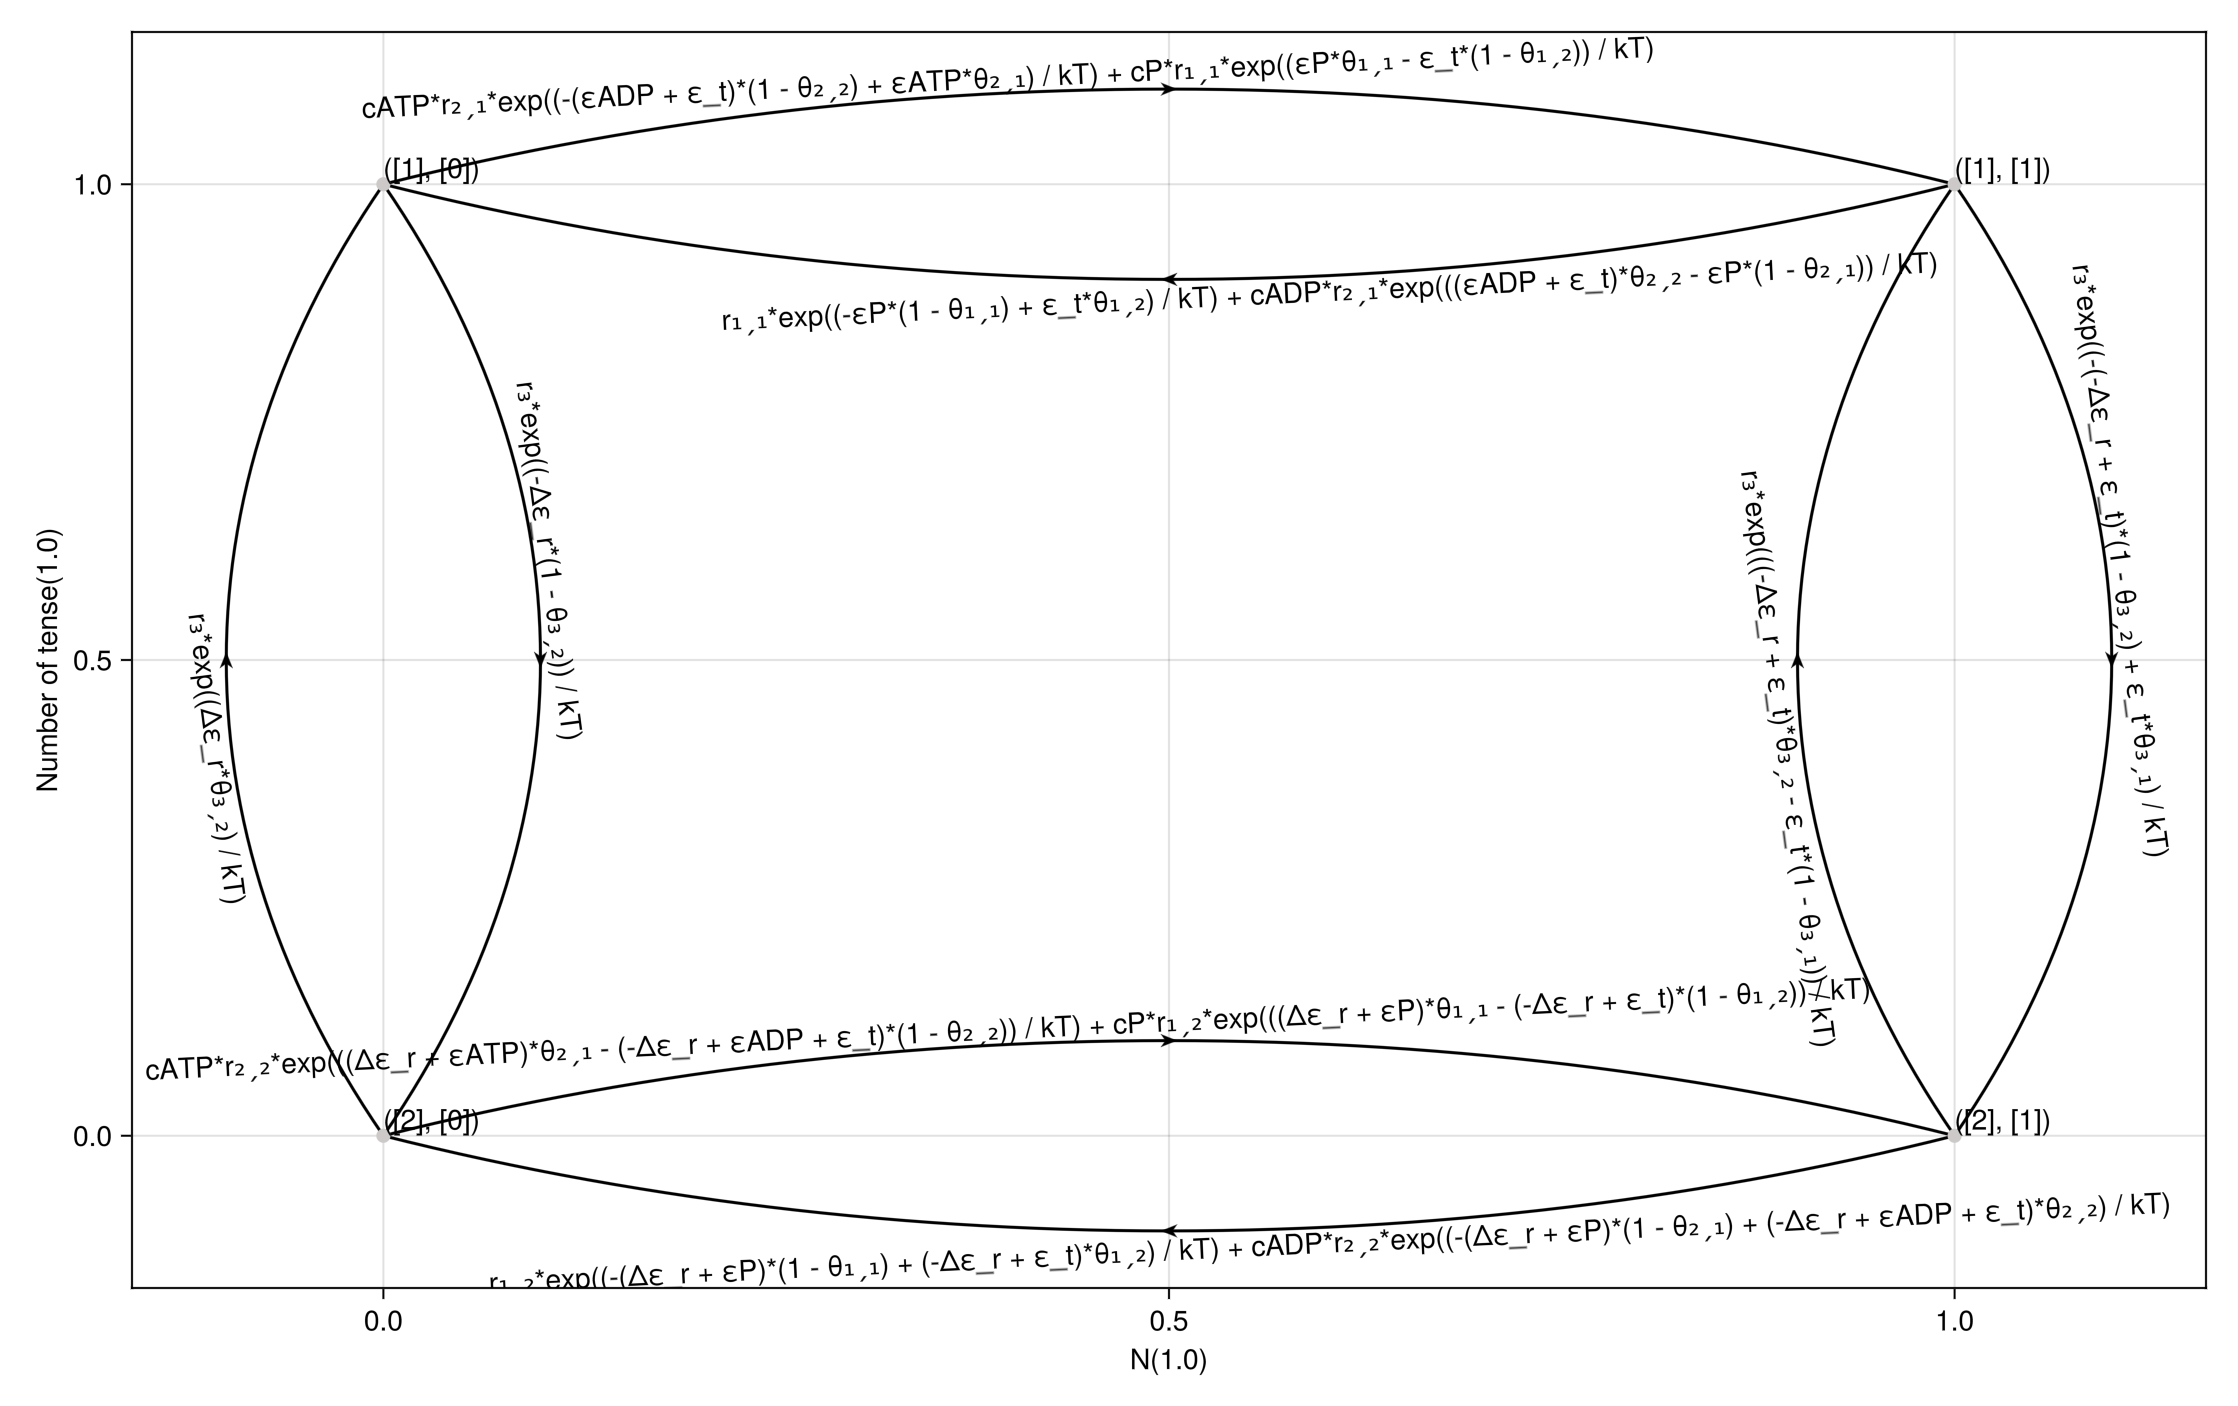
\includegraphics[width=\textwidth]{../../plots/symgraph_B=1_C=2_N=1_version=2.5.png}
    \caption{
        Diagram of single monomer transitions for $C=2,B=1$.
        Top row is the tense conformational states, bottom is the relaxed ones.
        Left column are without a ligand and right column with one ligand bound.
    }\label{fig:4sTs}
\end{figure}

As before the up and down transition (that change conformation) are naturally "driven" clockwise just due to the nature of the energies $\epsilon_t,\Delta\epsilon_r$.
\subsection{Systematic approach}\label{sec:fcsys}
Before we look at the exact rates for the $N=1$ system it is worth looking at the general picture of ligand binding by processes 1 and 2.
From \cref{eq:rp1} we can see that binding a ligand in process 1 is favoured as long as the energy is not raised by more than $\mu_P = \epsilon_P+\frac{1}{\beta}\ln(c_P)$
The same logic can be applied to process 2 and the results are summarized as
\begin{table}[H]
    \centering
    \begin{tabular}{c|c|c}
        Process & binding favoured if $\epsilon^{S'}_i-\epsilon^S_i<$ & overall rate scale \\
        \hline
        1 & $\mu_P = \epsilon_P+\frac{1}{\beta}\ln(c_P)$ & $r_1(c_i)$ \\
        \hline
        2 & $\mu_{ATP}-\mu_{ADP} = \epsilon_{ATP}-\epsilon_{ADP}+\frac{1}{\beta}\ln{\frac{c_{ATP}}{c_{ADP}}}$ & $r_2(c_i)$
    \end{tabular}
\end{table}
Coming back to the $N=1$ system, to complete the clockwise cycles from \cref{fig:4sTs} we want ligand binding to be favoured on the top edge where the energy difference $\epsilon^{S'}_i-\epsilon^S_i$ is $\epsilon_t$.
But we want it not to be favoured by the bottom edge where the energy difference is $\epsilon_t-2\Delta\epsilon_r$ which is always lower.
Thus it is impossible to have either of the processes favour binding in the top transition and favour debinding in the bottom one and so in order to complete the cycle we must use the dependence of the overall scales of the processes on the conformation.

So to complete the cycle, one of the processes must have its $\Delta\mu$ be $<\epsilon_t-2\Delta\epsilon_r<\epsilon_t$ and so favour debinding in both of the transtions.
And the other must have its $\Delta\mu > \epsilon_t > \epsilon_t-2\Delta\epsilon_r$ and so favour binding in both transitions.
Then we need to tune the overall scales of the rates $r_1, r_2$ as functions of the conformation so that we get the desired behaviour.

It seems plausible to choose process 1 as the one that favours debinding and process 2 as the energetically driven process that drives binding in the top process.
This gives as a bound on setting the $\Delta\mu$ which has two underlying degrees of freedom, we can either tune it using the chemical energies $\epsilon$ which may enter into both of the rates, or using the chemical concentrations which only affect the rate which has them used, these become the same when relevant $\theta_?$ are 1.
Next we still have to set the overall rate scales $r_{1/2}(c)$ for both monomer conformations.
It seems reasonable to have process 1 couple equally to both conformations, but to have process 2 couple stronger to the tense ($c_i=1$) conformation.

\subsection{Brute force approach}
To complete this cycle fully we get the conditions of
\begin{multline}
    c_P r_{1}(1) e^{\frac{\epsilon_P \theta_{1f} - \varepsilon_{t} \left( 1 - \theta_{1b} \right)}{kT}} + c_{ATP} r_{2}(1) e^{\frac{ - \left( \epsilon_{ADP} + \varepsilon_{t} \right) \left( 1 - \theta_{2b} \right) + \epsilon_{ATP} \theta_{2f}}{kT}} > \\
    r_{1}(1) e^{\frac{ - \epsilon_P \left( 1 - \theta_{1f} \right) + \varepsilon_{t} \theta_{1b}}{kT}} + c_{ADP} r_{2}(1) e^{\frac{\left( \epsilon_{ADP} + \varepsilon_{t} \right) \theta_{2b} - \epsilon_P \left( 1 - \theta_{2f} \right)}{kT}} \\
\end{multline}
\begin{align}
    c_{ATP} r_{2}(2) e^{\frac{\left( \Delta\varepsilon_{r} + \epsilon_{ATP} \right) \theta_{2f} - \left(  - \Delta\varepsilon_{r} + \epsilon_{ADP} + \varepsilon_{t} \right) \left( 1 - \theta_{2b} \right)}{kT}} + c_P r_{1}(2) e^{\frac{\left( \Delta\varepsilon_{r} + \epsilon_P \right) \theta_{1f} - \left(  - \Delta\varepsilon_{r} + \varepsilon_{t} \right) \left( 1 - \theta_{1b} \right)}{kT}} &< r_{1}(2) e^{\frac{ - \left( \Delta\varepsilon_{r} + \epsilon_P \right) \left( 1 - \theta_{1f} \right) + \left(  - \Delta\varepsilon_{r} + \varepsilon_{t} \right) \theta_{1b}}{kT}} + c_{ADP} r_{2}(2) e^{\frac{ - \left( \Delta\varepsilon_{r} + \epsilon_P \right) \left( 1 - \theta_{2ff} \right) + \left(  - \Delta\varepsilon_{r} + \epsilon_{ADP} + \varepsilon_{t} \right) \theta_{2b}}{kT}}
\end{align}

\subsection{Looking at the transition matrix}
We can also construct the transition rate matrix $R$ where $R_{ij}$ corresponds to the transition from $j$ to $i$.
This takes the form
\begin{align}
R \sim \begin{pmatrix}
0 & c & e & 0 \\
a & 0 & 0 & g \\
b & 0 & 0 & h \\
0 & d & f & 0 \\
\end{pmatrix} \qq{where states go as} \begin{pmatrix}
    (\set{1}, \set{0}) \\
    (\set{2}, \set{0}) \\
    (\set{1}, \set{1}) \\
    (\set{2}, \set{1})
\end{pmatrix}
\end{align}
where the variables are shorthands for the rates in \cref{fig:4sTs}.
We can symbolically solve for the eigenvalues of this matrix and have done so using wolfram, the results being
\begin{equation}
    \begin{pmatrix}
        -\frac{\sqrt{-\sqrt{(-a c-b e-d g-f h)^2-4 (a c f h-a d e h-b c f g+b d e g)}+a c+b e+d g+f h}}{\sqrt{2}} \\
        \frac{\sqrt{-\sqrt{(-a c-b e-d g-f h)^2-4 (a c f h-a d e h-b c f g+b d e g)}+a c+b e+d g+f h}}{\sqrt{2}} \\
        -\frac{\sqrt{\sqrt{(-a c-b e-d g-f h)^2-4 (a c f h-a d e h-b c f g+b d e g)}+a c+b e+d g+f h}}{\sqrt{2}} \\
        \frac{\sqrt{\sqrt{(-a c-b e-d g-f h)^2-4 (a c f h-a d e h-b c f g+b d e g)}+a c+b e+d g+f h}}{\sqrt{2}}
    \end{pmatrix}
\end{equation}

\section{Parameters}
The model has the following parameters
\begin{table}[H]
    \centering
    \begin{tabular}{c|c|c}
        Where they come from & parameters & units \\
        \hline
        Energy parameters & $\epsilon_t, \Delta\epsilon_r, \epsilon_b$ & \si{E} \\
        Equilibrium statistics & $\mu, \si{k_b}T$ & \si{E} \\
        Rates: overall scaling & $r_{1/2}(c_i),r_3$ -- $2C+1$ of these & rates -- \si{T^{-1}} \\
        Rates: dimensionless concentrations & $c_P,c_{ATP},c_{ADP}$ & \si{1} \\
        Rates: intrinsic chemical energies & $\epsilon_P,\epsilon_{ATP},\epsilon_{ADP}$ & \si{E} \\
        Rates: thetas/balancing & $\theta_{1/2/3,f/b}$ -- 6 of these & \si{1} \\
    \end{tabular}
\end{table}

\subsection{Reducing parameters}
Firstly, assuming constant $T$ we may choose $\si{k_B}T = 1\si{E}$ to be our energy unit.
We can also reasonably take all the $\theta_?$ to be equal.
Beyond this it gets more questionable.

\paragraph{Unit $\theta_?$}
We can start off with setting all the $\theta_?$ to one which is very convenient as that then makes the somewhat redundant degrees of freedom of the concentrations and intrinsic chemical energies have the same effect.
As such, with this simplification we can also withouth loss of complexity set all the intrinsic chemical energies to 0.

\paragraph{Rate scales $r_?$}
The absolute simplest scenario imaginable that can give the single monomer futile cycles as described in \cref{sec:fcsys} is where we have $r_1(?)=r_3=1$, $r_2(1)=1$ and $r_2(2)=0$.


\end{document}
